\subsection{Experiment 5: Sense v3 when the user cannot see the outcome}

Our WebShop user always knew whether a purchase was right, because we designed it to react to the outcome. Experiment 5 removes both conditions: $\tau^2$-bench's customer is not ours, and it cannot see whether its task was done, since the result lives in a database it never sees. There, learning from customer reactions taught the 1.7B agent to fail on the domains it practised, and even learning from the true outcome lowered its overall score.

Experiment 5 put the creature in $\tau^2$-bench's customer-service role, with Gemini 3 Flash playing the customer. Qwen3 0.6B and 1.7B each lived 30 days, 3 seeds per condition. Each day the agent served 30 customers from the airline and retail training tasks; each night it learned from the conversations judged good, either by the \emph{oracle} ($\tau^2$-bench's own check of the final database) or by the frozen \emph{sense v3} reading how the customer ended the conversation. Every 3 days it sat an exam on the official test tasks, never learned from: airline (20), retail (40) and telecom (40), a domain it never practised.

\textbf{Without learning.} The plain models solved a few tasks in each domain: 0.6B 5\% of retail, 35\% of airline and 33\% of telecom; 1.7B 18\%, 25\% and 35\% (in a separate baseline run; the 1.7B lives' own day-0 exams averaged 11\% on retail, as in the table below); 4B, for reference, 16\% (on the 32 retail tasks that ran without error), 20\% and 30\%. Retail separates the sizes best, because every success needs 4-16 correct tool calls. Some airline successes are tasks where the right answer is to refuse, and many telecom successes need one agent action while the customer fixes their own phone.

\textbf{The customer cannot judge.} Before any learning, we let sense v3 read how the 292 baseline conversations ended and compared its verdict with the true outcome. 20 of its 34 yeses came after failed tasks. The sense read the customers correctly: they ended with clear, sincere thanks, for example ``Alright, that's great, thanks a lot.'' But the customer cannot see the database, so it often thanks the agent after a wrong payment method, a broken rule or a missed detail. Retail separated well (a yes after 50\% of done tasks, 6\% of failed ones); airline did not (6\% against 30\%).

\textbf{Learning from reactions collapses.} In the lives, it was worse. Only 20\% of the conversations sense v3 accepted had in fact succeeded (47 of 232 for 1.7B, 42 of 212 for 0.6B), and sense v3 missed most real successes, learning from 10-20\% of them. All three 1.7B \emph{sense v3} lives ended far below where they started on day 30 (2\%, 0\% and 11\% over all exam tasks): airline 25\% to 2\%, retail 11\% to 3\%, telecom 33\% to 8\%; over all exam tasks they fell from 23\% to 4\% (paired t-test over the 3 lives, p = 0.03). The \emph{oracle} lives fell too: over all exam tasks the 1.7B \emph{oracle} lives went from 23\% to 13\% and the 0.6B ones from 21\% to 13\%, and the 0.6B \emph{sense v3} lives (21\% to 15\%) ended above the 0.6B \emph{oracle}. With 3 lives per condition, the day-30 gap between the 1.7B \emph{sense v3} and \emph{oracle} lives (4\% against 13\%) is not significant (p = 0.12). The clear difference is on 1.7B airline, which both conditions practised: the \emph{oracle} lives all ended at 35\%, the \emph{sense v3} lives averaged 2\% (6\%, 0\% and 0\%). We ran no life without learning on $\tau^2$-bench, so every fall here is against the life's own day 0. One stopped completing tasks within nine days: its practice success fell from 17\% in days 1-5 to under 1\% in days 21-25, while its conversations grew longer, from about 15 to 22 agent turns. The 0.6B \emph{sense v3} lives survived because they learned little, about 2 conversations a day; their airline and retail scores did not move, and telecom fell in one of the three.

\textbf{Example 2: a thanked failure (Experiment 5, 1.7B \emph{sense v3} life, day 2).} A customer asked to cancel all their upcoming flights. The agent did not complete the task (reward 0). The customer ended: ``C'est parfait. Merci pour votre aide. That is all I needed.'' Sense v3 scored it 100 with confidence 0.99, and it became a lesson.

\textbf{A second observation: correct lessons, lopsided.} The \emph{oracle}'s lessons were all correct, yet the overall score fell. About three quarters came from airline (72\% for 1.7B, 77\% for 0.6B), where the small models succeed more often, although retail has more than twice as many training tasks. The 1.7B \emph{oracle} lives rose on airline from 28\% to 35\% (all three ended at 35\%), fell on retail from 11\% to 6\%, and fell on telecom from 32\% to 10\%. Telecom fell in all 6 \emph{oracle} lives, by more than 10 points in four of them, three of those to 0-3\%. Narrowing of this kind could only show here: on WebShop every task is the same kind of task.

\begin{figure}[htbp]
\centering
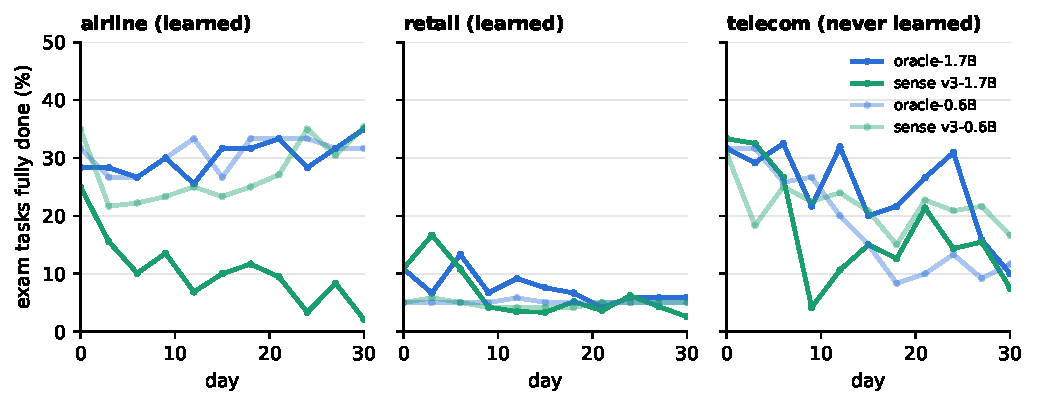
\includegraphics[width=1.0\linewidth]{figures/fig5_tau2_domains}
\caption{Experiment 5, 3 seeds per condition; exams on day 0 and every 3 days; broken exam conversations left out. \emph{Oracle} lessons moved skill to airline while retail and telecom fell; the 1.7B \emph{sense v3} lives collapsed.}
\label{fig:5}
\end{figure}

\begin{center}\small
\begin{tabular}{@{}
  >{\raggedright\arraybackslash}p{(\linewidth - 10\tabcolsep) * \real{0.1565}}
  >{\raggedright\arraybackslash}p{(\linewidth - 10\tabcolsep) * \real{0.1565}}
  >{\raggedright\arraybackslash}p{(\linewidth - 10\tabcolsep) * \real{0.1565}}
  >{\raggedright\arraybackslash}p{(\linewidth - 10\tabcolsep) * \real{0.2000}}
  >{\raggedright\arraybackslash}p{(\linewidth - 10\tabcolsep) * \real{0.1217}}
  >{\raggedright\arraybackslash}p{(\linewidth - 10\tabcolsep) * \real{0.2087}}@{}}
\toprule\noalign{}
\begin{minipage}[b]{\linewidth}\raggedright
Condition
\end{minipage} & \begin{minipage}[b]{\linewidth}\raggedright
Airline (learned)
\end{minipage} & \begin{minipage}[b]{\linewidth}\raggedright
Retail (learned)
\end{minipage} & \begin{minipage}[b]{\linewidth}\raggedright
Telecom (never learned)
\end{minipage} & \begin{minipage}[b]{\linewidth}\raggedright
Lessons a day
\end{minipage} & \begin{minipage}[b]{\linewidth}\raggedright
Lessons truly successful
\end{minipage} \\
\midrule
\emph{oracle} 1.7B & 28 $\rightarrow$ 35 & 11 $\rightarrow$ 6 & 32 $\rightarrow$ 10 & 5.3 & 100\% \\
\emph{sense v3}, 1.7B & 25 $\rightarrow$ 2 & 11 $\rightarrow$ 3 & 33 $\rightarrow$ 8 & 2.6 & 20\% \\
\emph{oracle} 0.6B & 32 $\rightarrow$ 32 & 5 $\rightarrow$ 5 & 32 $\rightarrow$ 12 & 5.2 & 100\% \\
\emph{sense v3}, 0.6B & 35 $\rightarrow$ 35 & 5 $\rightarrow$ 5 & 31 $\rightarrow$ 17 & 2.4 & 20\% \\
\bottomrule
\end{tabular}
\end{center}

Share of exam tasks fully done, day 0 $\rightarrow$ day 30, mean of 3 seeds. Exams are small: one airline task is 5 points, one retail or telecom task 2.5, so moves under about 10 points are within noise. Exam conversations that broke, for example a loop past the length limit, are left out; counting them as failures would lower the collapsed lives further. The 0.6B barely moved on retail: every 0.6B life scored exactly 5\% on day 0 and on day 30, and 59 of its 66 retail exams scored 5\%.
